\chapter{Struttura}
   In questo capitolo verranno descritte le apparecchiature utilizzate per il progetto.
\section{ROS}
	ROS, acronimo per Robot Operating System, \`e un insieme di librerie software e strumenti che facilitano la creazione di applicazioni orientate alla robotica; inoltre \`e completamente open source in modo da incentivare la collaborazione tra i vari utilizzatori.
	
	ROS \`e ufficialmente supportato solo sul sistema operativo Ubuntu, ma fornisce anche supporto a svariate piattaforme hardware come manipolatori, robot mobili e robot umanoidi.
	
	In ROS ogni applicazione viene definita nodo; ogni nodo comunica con altri nodi attaverso tre protocolli: Topic, Service e Action.
	
	I Topic sono dei canali di comunicazione con cui i nodi possono scambiarsi messaggi; quando un nodo publica un messaggio su un topic tutti i nodi sottscritti a tale topic vengono notificati della presenza di un messaggio ed eseguono determinate operazioni utilizzando le informazioni fornite dal messaggio.
	
	Il concetto di Service si basa sulla necessit\`a di un sistema distribuito di avere delle interazioni richiesta/risposta; tramite un Service un nodo può richiedere che un altro nodo esegua un determinato compito e comunichi al richiedente un eventuale risultato.
	
	Il protocollo di Action \`e fondamentalmente uguale a quello di Service, ma è stato esteso in modo da fornire al richiedente la possibilit\`a di annullare la richiesta nel caso in cui questa impieghi un tempo eccessivo per essere portata a termine.
	
	Questi tre protocolli consentono di realizzare applicazioni per qualunque necessit\`a in ambito di robotica.
	
\section{Robot Mobili e-Puck}
	I robot mobili e-Puck sono dei robot mobili a due ruote di dimensioni compatte dotati di una grande variert\`a di sensori e possono essere usati in svariate applicazioni che spaziano dalla robotica mobile a sistemi biologici e di intelligenza artificiale.
	
	
	\begin{figure}[h]
	\centering
	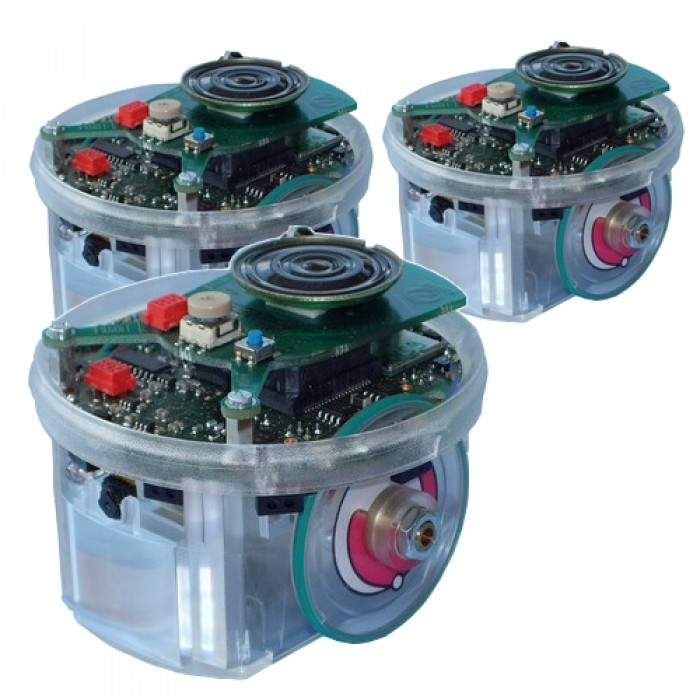
\includegraphics[width=4cm]{images/epuck}
	\caption{Robot e-Puck\label{epuck}}
	\end{figure}
	
	\subsection{Sensori}
	Gli e-Puck sono dotati di 8 sensori di prossimit\`a, un accelerometro 3D, 3 microfoni omni-direzionali, una fotocamera VGA e uno speaker
	
	\subsection{Ruote}
	Le ruote sono coassiali e comandate separatamente da due motori passo-passo attraverso un riduttore meccanico con rapporto di trasmissione 1/50.
	\begin{figure}[h]
	\centering
	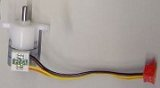
\includegraphics[width=4cm]{images/motor+cable}
	\caption{Motore passo-passo con riduttore\label{motore}}
	\end{figure}
	\subsection{Controllore}
	Il sistema \`e comandato da un microcontrollore dsPIC con clock a 60MHz e un DSP per processare i segnali.
	\begin{figure}[h]
	\centering
	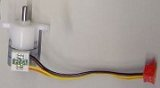
\includegraphics[width=4cm]{images/motor+cable}
	\caption{Motore passo-passo con riduttore\label{motore}}
	\end{figure}
	
	\subsection{Connessioni}
	Il micro controllore fornisce due connessioni uart; la prima collegata a un chip Bluetooth e la seconda disponibile fisicamente attraverso un connettore micromatch.
	La connessione Bluetooth avviene attraverso un chip  LMX9820A prodotto da National Semiconductor; questo chip fornisce uno stack Bluetooth completo e compatibile con la versione 1.1.
	Per facilit\`a di utilizzo si \`e scelto di utilizzare la connessione senza fili per comunicare con i robot, in particolare si \`e scelto il protocollo RFCOMM, tale protocollo \`e usato per generare un flusso virtuale di dati seriali, simulando dunque i segnali di controllo dello standard RS232 fornendo una connessione seriale fittizia.
	
	La connessione a lato computer avviene utilizzando due adattatori Bluetooth Logilink compatibili con lo standard 4.0 e retrocompatibili, dunque adatti ad essere utilizzati con i robot scelti.
	La tecnologia Bluetooth fornisce un indirizzo univoco a 3 bit ad ogni dispositivo collegato alla rete, siccome un dispositivo deve essere denominato master (nel nostro caso gli adattatori) rimangono solo 7 indirizzi disponibili per altri dispositivi, non sufficienti a connettere contemporaneamente tutti e 8 i robot disponibili; per questo motivo si \`e scelto di utilizzare due adattatori, creando così due sottoreti ed estendendo il numero di connessioni simultanee di robot al computer fino a 14.
	L'utilizzo di due adattatori fornisce inoltre il vantaggio di eliminare il collo di bottiglia provocato dalla limitata velocit\`a di trasmissione di una singola antenna Bluetooth.
	\begin{figure}[h]
	\centering
	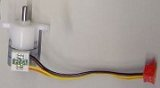
\includegraphics[width=4cm]{images/motor+cable}
	\caption{Schema delle connessioni Bluetooth\label{Bt}}
	\end{figure}
\clearpage	   	
\section{Arena}
	Tutte le simulazioni sono effettuate all'interno di un'arena composta da un piano, sul quale i robot si possono muovere, e da una struttura metallica a forma di L.
	
	\begin{figure}[H]
	\centering
	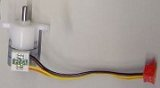
\includegraphics[width=4cm]{images/motor+cable}
	\caption{Arena con la struttura di supporto per la webcam \label{arena}}
	\end{figure}
		
	Per sostenere una webcam Logiteck QuickCam Pro 9000 dotata di un sensore con risoluzione di 2.0 Megapixel con il compito di acquisire le immagini dei robot in movimento sul piano e consentire al computer di elabrare le immagini per rilevare la posizione dei singoli robot sull'arena.
	La webcam viene collegata al computer tramite un cavo USB 2.0 
	
	

\iffalse
	
\section{Grassetto, Italico e amenit\`a varie}
   \`E banale ottenerli (a differenza della ``e'' maiuscola e
   accentata quando usate qualcosa di diverso dal \LaTeX2),
   gi\`a che ci siamo potete anche vedere come si
   ottiene una lista e un nota a pi\`e di pagina:
   \begin{itemize}
   \item \textbf{Grassetto}
   \item \emph{Italico}
   \item \textsc{Maiuscoletto}
   \item \texttt{Macchina da Scrivere}\footnote{In genere \`e conveniente non
                 abusare troppo di questo, visto che \`e gestito male nei rientri a capo.}
   \end{itemize}
\section{Tabelle}

   Per spaventarvi subito guardate un po' come si ottiene la tabella~\ref{miatabella}.
   \begin{table}[h!]
    \centering
    \begin{tabular}{|l|c|c|}
    \hline
    Oggetto & Costo & peso \\
    \hline
    \hline
    Pere    & 123   & 345  \\
    \hline
    Mele    & 234   & 56   \\
    \hline
    \end{tabular}
    \caption{Tabella di esempio\label{miatabella}}
   \end{table}

\section{Figure}
   Molto pi\`u semplice inserire la figura~\ref{miafigura}
   generata usando \texttt{xfig} (ottimo programma
   per fare disegni da inserire in relazioni/tesi). 
   \begin{figure}
   \centering
   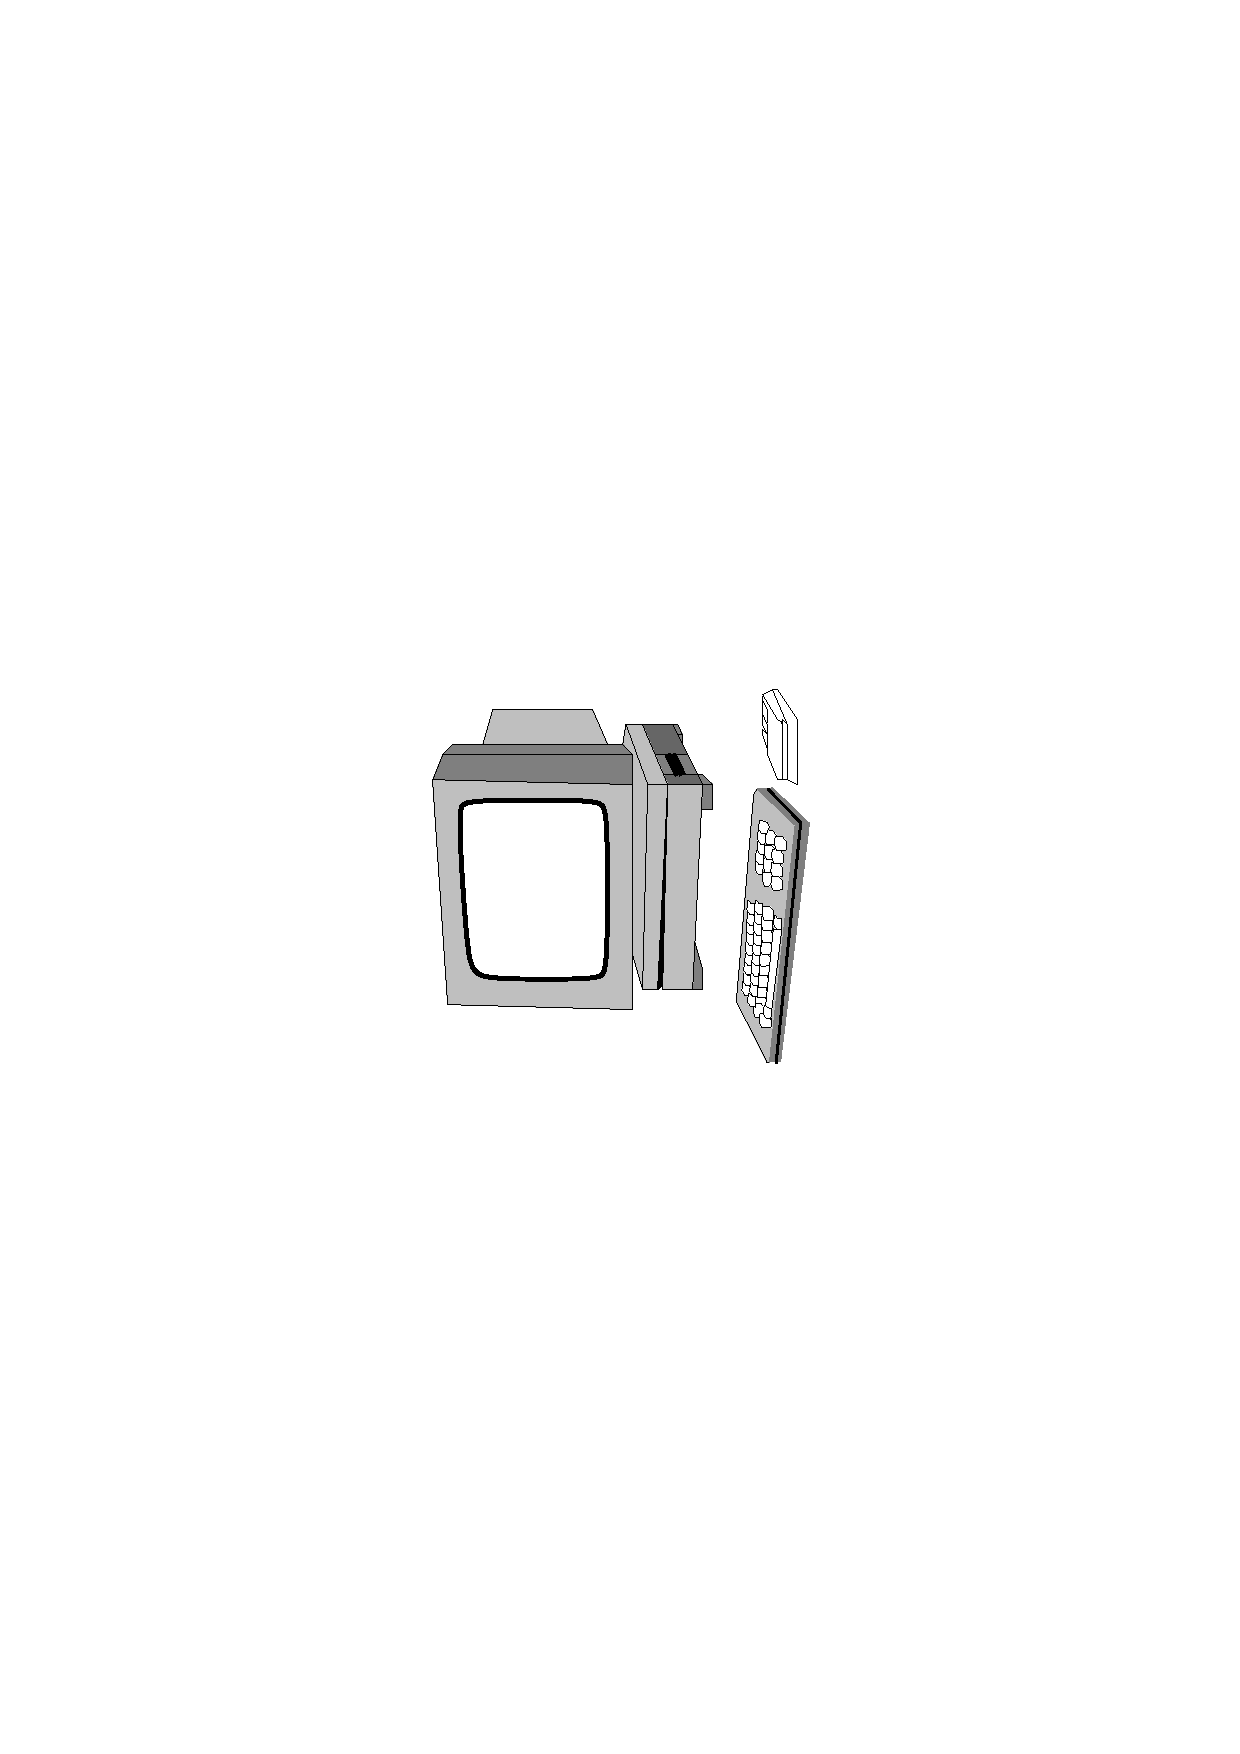
\includegraphics[width=4cm]{images/esempio}
   \caption{Esempio di figura\label{miafigura}}
   \end{figure}

\section{Equazioni}
   Le equazioni sono facilmente ottenibili, per esempio
   osservate nel sorgente $f(x)=x^{2}_{ij}\times \frac{(x+2)}{4}$
   oppure il suo equivalente~\ref{myeq} ottenuto utilizzando l'ambiente
   \emph{equation}:

   \begin{equation}
   \lim_{n \to \infty}
   \sum_{k=1}^n \frac{1}{k^2}
   = \frac{\pi^2}{6}
   \label{myeq}
   \end{equation}

\section{Lettere accentate\label{accenti}}

   Il \LaTeX2\/
   le gestisce benissimo: àèìòùÀÈÌÒÙáéíóúÁÉÍÓÚ (se avete l'accortezza di salvare i file con codifica \texttt{UTF-8}
   ma le nostre tastiere un po' meno\footnote{in realt\`a a volte l'ALT di destra
   usato con la vocale opportuna o il tasto sopra/sottostante (con eventualmente lo
   shift per le maiuscole) produce i vari tipi di accento (acuto, ottuso, dieresi\ldots).},
   allora in questo caso si usa:
   \`a\`e\`{\i}\`o\`u\`A\`E\aa\v e e cos\`{\i} via...
   \newpage
   Comunque per avere maggiori informazioni leggetevi la guida \emph{The Not So Short Introduction to \LaTeX2}
   che trovate gi\'a stampata da qualche parte nei laboratori.

\section{La Bibliografia}

   Per la gestione semplice e intuitiva della bibliografia si usa un programma
   aggiuntivo, il \BibTeX. A tal fine provate a dare il comando
   \texttt{bibtex tesi} e poi ri-latexxare due volte\footnote{se non funziona
   probabilmente non vi siete copiati i file local.bib e public.bib.}.
   Usando xdvi potrete notare che \`e stata completata la bibliografia
   e inserite le seguenti citazioni~\cite{sql,cv1,itsc99,mpi-boselli,mpipov,isata99,spie99,ipps99,iv98-1,iv98-2,spie98,isata97,iv97,camp97,canpc,ica3pp97,eusipco96,iv96,icip96}

   Per capire come \`e stato ottenuto il tutto guardate il sorgente, 
   provate poi ad osservare i file .bib per capire come aggiungere materiale da
   citare (il tutto \`e comunque spiegato in~\cite{btxdoc})\footnote{In realt\`a
   \`e decisamente conveniente includere file di bibliografie gi\`a esistenti.
   Per esempio,
   la maggioranza di voi hanno gi\`a definita una variabile BIBINPUTS che punta, tra le altre cose, ad
   alcune directory dove esistono alcuni file .bib che \`e gi\`a possible
   includere. Sicuramente il vostro co/relatore ha una directory in cui sono contenuti
   uno o pi\`u file .bib con le citazioni che fanno al vostro caso, fatevela dire
   e modificate la variabile di ambiente BIBINPUTS (nel file .user-cshrc) aggiungendo
   il \emph{path} opportuno.}

   Dal nostro sito web (area studenti) è possibile scaricarsi il database in formato \BibTeX di
   tutte le tesi sperimentali dal 1990 ai giorni nostri.
\fi


